\documentclass{article}

\linespread{1}
\usepackage[utf8]{inputenc}
\usepackage[left=1.5in,right=1.5in,bottom=1in]{geometry}
\setlength\parindent{0pt}
\setlength{\parskip}{1em}
\setcounter{secnumdepth}{0}
\usepackage{outlines}
\usepackage{graphicx}
\graphicspath{ {imgs} }
\usepackage{hyperref}
\usepackage{color,soul}

\usepackage[
backend=biber,
style=apa,
citestyle=authoryear,
sorting=nyt,
]{biblatex}
\addbibresource{refs.bib}

\usepackage{comment}
\specialcomment{topicsen}{\begingroup\bfseries\scriptsize}{\endgroup}
%\excludecomment{topicsen}

\newcommand{\alignedmarginpar}[1]{%
        \marginpar{\raggedright\small #1}
    }

\title{Principles of Urban Planning and Urbanism}
\author{Carla Hyenne}

\begin{document}

\maketitle

\tableofcontents

\pagebreak

yellow = urban planning

\section{Mesopotamia}

...

%%%%%%%%%%%%%%%%%%%%%%%%%%%%%%%%%%%%%%%%%%%%%%%%%%
\section{Planning the Ancient City}
%%%%%%%%%%%%%%%%%%%%%%%%%%%%%%%%%%%%%%%%%%%%%%%%%%

\subsection{Greek Urban Planning}
...

\subsection{Roman Urban Planning}

\textit{March 15th 2022}

Volterra, Tuscany: an Etruscan city in 7th century BC shows a grid system with large avenues.

Rome's Golden Age lasted 200 years, from 50BCE to 150CE\alignedmarginpar{(Before) Common Era}. It was an unplanned city which gradually improved. The site of Rome was on hills in a flood-prone low-land, and flooding levels were engraved on building walls.


The first priority for such a large city as Rome, was to get rid of the sewage which is a health hasard. \textit{Cloaca Maxima} was introduced as the sewer of Rome.

The second priority was water, for which aqueducts were built (first in 312). The system was not water efficient, and the volume of water that flowed was much more than necessary. 14 aqueducts were built, delivering 1 billion litres/day. It flowed continuously because they didn't have proper taps, no water storage, and aqueducts were not pressurised. Since water flowed in the streets, the sidewalks were high and raised pavement stones served as crosswalks.

The third concern was food. Daily food doles were distributed, pork and 1.4kg of bread. 

Infrastructures like the forum, Colosseum and city walls were built and expanded under different emperors. 

Housing was socially mixed, and to accommodate the population growth, buildings were built wit additional stories (from 3 stories in 3rd century BCE to 5 stories in 1st century BCE). These constructions became unstable due to the additional weight, even though they were built from solid brick.
Residential buildings had an enclosed patio. The ground floor had shops and storage rooms, and people lived above.
The city is noisy, dark at night, and polluted.

\subsubsection{Pompeii}

An unplanned old town, and a planned new city. They had the same raised sidewalks and crossing stones to avoid the flowing water, housing with atriums.

\subsubsection{Novaesium, a Legion's Camp}

Novaesium, or Neuss, is a city in North-Rhine-Westphalia near Düsseldorf, with many Roman sites.

The camps had exactly the same layout so that soldiers would always find their way around. There were regulations on where and how bathrooms, for eg., should be built.
They were built on elevated grounds to avoid flooding like in Rome. They were built along the Danube (from the Rhine, down to the Black sea) which created a boundary. 

Outside the camp, there were civilian settlements around, which ca be seen in Vienna's city centre.

\subsubsection{Ancient cities in contemporary knowledge}

What is the point of this knowledge nowadays? Tourism and events, but also urban imaginaries. Knowledge is being recycled to create importance and awareness in the city.

%%%%%%%%%%%%%%%%%%%%%%%%%%%%%%%%%%%%%%%%%%%%
\section{Planning the Medieval City}
%%%%%%%%%%%%%%%%%%%%%%%%%%%%%%%%%%%%%%%%%%%%

\subsection{From the Roman Empire to the Middle Ages}

The Dark Ages lasted between 500-1000 AD, and was a period of time between the Roman Empire and the Middle Ages. During the Dark Ages, much of the former powers disappeared (the Roman Empire disintegrated, which cut off trade routes and information flows except for the oriental merchants\alignedmarginpar{Orient = non-Latin speaking}), technologies were lost, cities shrank and disappeared (eg. Trier, Cologne, Avenches). 

The `Ancient World' was fragmented into islands of small-scale, manorial feudalism, protected by fortifications and castles. $\rightarrow$ shrinkage, caused by ch

\subsection{Early Middle Ages}

...

\subsection{High Middle Ages}

Cities in the High Middle Ages have 6 origins:

\begin{enumerate}
	\item \textbf{Rebuilding} on top of, and with, Roman remains. They were former Roman cities, blossoming again as residences of Emperors (Aachen), Archbishops (Trier, Regensburg, Cologne) and Dukes (Vienna)
	\item \textbf{Monastery} settlements with Bishop's seat (Bamberg, Kaptol)
	\item \textbf{Castles} of the Principality (bourg) combined with settlement for craftsmen and merchants (faubourg, portus, Graz)
	\item \textbf{Commercial settlements} of free merchants and craftsmen, developed from wik settlements (merchant settlements), Germanic-Slavic origins
	\item Free manors and \textbf{Market-towns} (Ackerbürgerstädte)
	\item Newly-founded \textbf{mining towns}, based on better knowledge of where coal, gold, may be found (Frankenberg, Sachsen, Freiberg (DE), Banska Stiavnica (Slovakia)...)
\end{enumerate}

\subsection{Characteristics of Medieval Cities}

\begin{outline}
	\1 City walls date from the Middle Ages, to protect against barbaric attacks, and a castle located higher on a hill
	\1 Ditches around the city (graben)
	\1 Narrow streets with burgher houses
	\1 Church (goes without saying, a Christian endeavour)
	\1 Central market square, need to feed the growing population
\end{outline}

Almost all European cities date from the High Middle Ages, and European city tourism is exploiting these legacies.

\subsubsection{High Medieval City}

\textit{ref. Vance chapter 4}

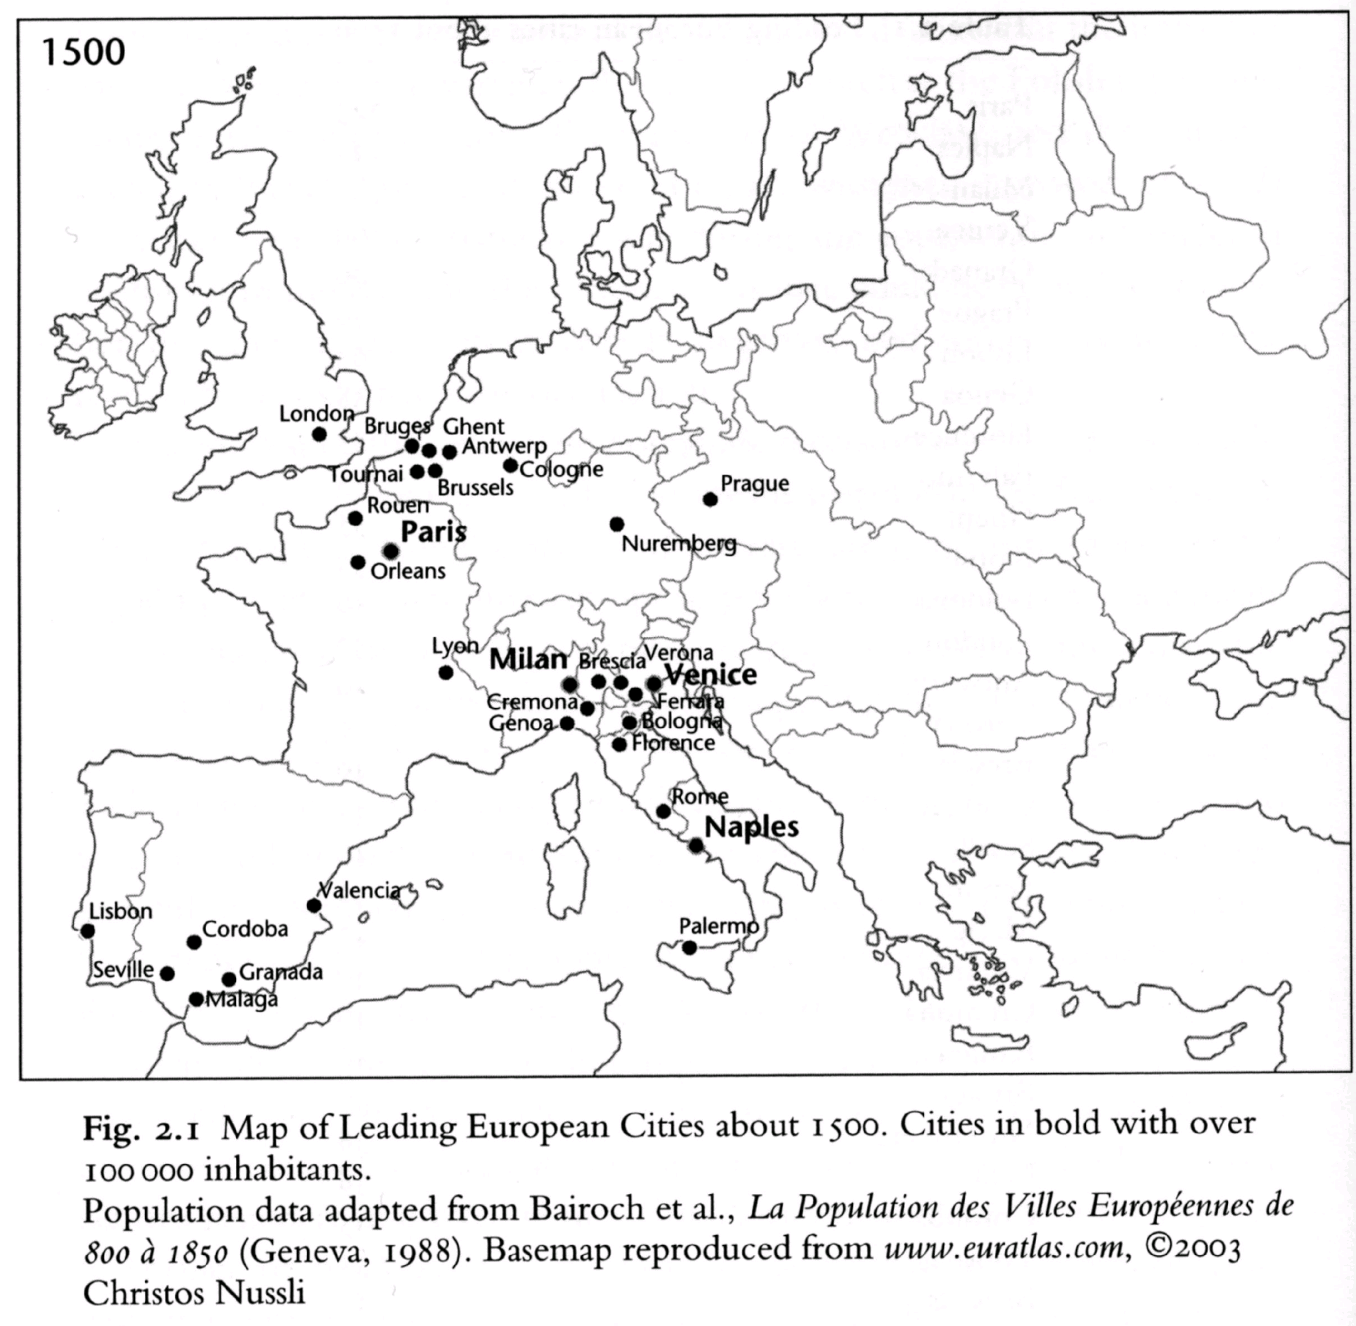
\includegraphics[width=\textwidth]{leading_cities_1500}

There is an upswing around 1200 AD (eg. Notre Dame 1163-1345). New Towns are founded and Ancient Towns are renewed. There is a strict separation of urban and rural functions\alignedmarginpar{ref. Max Weber}. There are two types of urban places:

\begin{outline}
	\1 Natural settlements: local market based central places, and
	\1 Systemic settlements: long distance trade based, with varying degree of freedom from Feudal powers
\end{outline}

There are two hearths of Medieval urbanism, Flanders and North Italy (Po Basin and Tuscany). Flanders and North Italy are ``trade-originating Europe'', with systematic settlements, and the rest is ``trade-supporting Europe'' with natural settlements that depend on their role as central places.

Until today, both functions are important for a city to prosper: its role as a shopping and service centre for its region, and its ``global city''-ness, based on its worldwide connectivity in services and goods.

There are two basic types of architecture:

\begin{outline}
	\1 Mediterranean: uninterrupted urban tradition
	\1 North of the Alps: new foundations and many new settlers
\end{outline}

\subsubsection{Mediterranean City}

Unlike the ancient city, housing combines work and home due to a scarcity of space in the Medieval City. The houses are narrow burgher house-shops, or even house-towers built from local materials (stone, timber, adobe, studwork).

Conflicts between factions meant that structures like house-towers were built.

Remains of previous architecture can be traded as vernacular architecture (concerned with domestic and functional, and not public and monumental). Places like amphitheatres are recycled, along with their building materials.

The Mediterranean city is a city of \textbf{factions} (house towers of Bologna, Lucca). It is a mix of Renaissance palaces, earliest tenement houses and individual houses, many arcades.

The Black Death pandemics (1348) more than halves the population of cities. 

\subsubsection{North of the Alps}

The city North of the Alps is a city of \textbf{guilds}. 

There are no City-States bordering each other, but (temporarily) Free Cities surrounded by feudal countryside. There is a stark contrast between urban and rural society.

There are two settlement systems, ``central-place'' and ``mercantile''. There's functional segregation based on guilds (unlike Mediterranean cities of `factions').
Merchants are clustering at ``portus'' and then expanding.

The nobility still remains in their countryside castles (unlike Mediterranean cities where the nobility returned earlier). 

Tall house-shops, on narrow burgage plots, within tight city walls, catering for an extended family (including apprentices and journeymen).

``Quarters of Tolerance'' for the outsiders like merchants, students...

\subsection{Timeline of Medieval Cities}

Similar to Ancient cities, from ``geomorphic'' unplanned cities (type 1), evolving into more and more ``geometric'' for newly-founded planned cities, particularly in Central and Eastern Europe.

\begin{enumerate}
	\item Unplanned cities (1100 AD)
	\item Rebirth of the planned city
	\item Zähringer's cross-shaped market towns
	\item Towns with long market-streets
	\item Towns with ladder-type streets
	\item Rebirth of the grid city
	\item The grid-shaped town (13th century)
\end{enumerate}

%%%%%%%%%%%%%%%%%%%%%%%%%%%%%%%%%%%%%%%%%%%%
\section{Planning the Absolutist City}
%%%%%%%%%%%%%%%%%%%%%%%%%%%%%%%%%%%%%%%%%%%%

\subsection{}

%%%%%%%%%%%%%%%%%%%%%%%%%%%%%%%%%%%%%%%%%%%%
\section{Fighting the Evils of the Early Industrial City}
%%%%%%%%%%%%%%%%%%%%%%%%%%%%%%%%%%%%%%%%%%%%

\subsection{}

%%%%%%%%%%%%%%%%%%%%%%%%%%%%%%%%%%%%%%%%%%%%
\section{Urban Engineering and Fin de Siècle Urbanism}
%%%%%%%%%%%%%%%%%%%%%%%%%%%%%%%%%%%%%%%%%%%%

\subsection{}

%%%%%%%%%%%%%%%%%%%%%%%%%%%%%%%%%%%%%%%%%%%%
\section{Reformist Urbanism}
%%%%%%%%%%%%%%%%%%%%%%%%%%%%%%%%%%%%%%%%%%%%

\subsection{}

%%%%%%%%%%%%%%%%%%%%%%%%%%%%%%%%%%%%%%%%%%%%
\section{Modernism, under both Capitalism and Socialism}
%%%%%%%%%%%%%%%%%%%%%%%%%%%%%%%%%%%%%%%%%%%%

\subsection{}

%%%%%%%%%%%%%%%%%%%%%%%%%%%%%%%%%%%%%%%%%%%%
\section{The Local Welfare ``State''}
%%%%%%%%%%%%%%%%%%%%%%%%%%%%%%%%%%%%%%%%%%%%

\subsection{}

%%%%%%%%%%%%%%%%%%%%%%%%%%%%%%%%%%%%%%%%%%%%
\section{The Neoliberal City and its Limits}
%%%%%%%%%%%%%%%%%%%%%%%%%%%%%%%%%%%%%%%%%%%%

\subsection{}

%%%%%%%%%%%%%%%%%%%%%%%%%%%%%%%%%%%%%%%%%%%%
\section{The Sustainable City}
%%%%%%%%%%%%%%%%%%%%%%%%%%%%%%%%%%%%%%%%%%%%

\subsection{}


%%%%%%%%%%%%%%%%%%%%%%%%%%%%%%%%%%%%%%%%%%%%
\section{Readings}
%%%%%%%%%%%%%%%%%%%%%%%%%%%%%%%%%%%%%%%%%%%%

\subsection{Ancient City}

\subsubsection{Rome: \textit{The Establishment of the Urban Order, The Imperial City} \parencite{hall1998cities}}

\begin{outline}
	\1 Ancient Rome was the first mega city, estimated at 1 million people. Although it wasn't extremely technologically advanced, its success (in terms of population, and power I guess) is in part due to its urban infrastructure and developments
	\1 It was an extremely unequal society
	\1 Rome had features we recognise in modern cities: dense living spaces with (abusive) landlords, courts, theatres, basilicas, large gathering spaces (colosseum), forums, sewage systems,...
	\1 Housing conditions
		\2 Apartments were a hasard, because they were made of wood and we prone to fires. Rome had `vigils' who were firemen and looked out for fires. Some kind of red clay bricks were banned because they were not sturdy enough building materials
		\2 Richer households had more luxurious houses, but the comforts were still limited (eg. most lacked running water). Rich people purchased agricultural land outside the (western side?) of the city, which limited sprawl because the fields were in the way
	\1 Shops and baths
		\2 Baths were incredibly noisy place and a ``social necessity'' (p. 631), and emphasised the importance of a water system. Acquaducts were built to serve them. Baths started as privately run places, then came enterprises, and then came public baths
		\2 The streets were super narrow (2.9m wide), and always congested. Some streets were pedestrian only, and the rich travelled in cushioned chairs (sedan chairs) carried by men
		\2 Days were divided into 12 hours: first hour at sunrise, midday when sun was highest, and last hour at sunset. Thus hours were longer during the summer, and shorter during the nigh
	\1 Two main and complex challenges for Rome: to feed and water its large population. It managed to do both, even though it might not have been done the most efficiently
	\1 Water
		\2 Aqueducts were built to supply the city with water, supplying up to 1 billion litres of high quality water daily. Distribution is estimated to have been: 26\% for the emperor's service area, 32\% public use, 44\% private use. They were expensive to build and run, and a team of people were appointed to keep them running and maintained
		\2 Households used 60 times more water then, than today's standards, which was attributed mostly to the baths. Overflow water from public fountains was used to clean the streets, beneficial because there was no sewage system, and fountains also served to cool the city in the hot summers
	\1 Funding
		\2 Aqueducts were expensive and land had to be bought, and mostly funded through war booty (Rome fought many wars, in Europe, North Africa, Asia...), also through selling land
	\1 Sewers
		\2 People emptied their chamber pots outside, and thus residential areas didn't smell nice. The city relied on the heavy inflow of water through the aqueducts to dilute the sewage enough that it wouldn't be a problem when it arrived in the rivers/sea
	\1 Health
		\2 Average life expectancy was 27, infant mortality rates were 20\%, and there was a class difference in life expectancy: the poor lived 20, the rich 30, mostly because the poor didn't have enough to eat, and the living conditions spread diseases (cholera, plague, malaria...)
	\1 Food
		\2 Rome wasn't abundant in food, and didn't drain food products from the surrounding regions as can be seen with urbanisation trends in North Africa, for example (p. 649). It took a long time to travel (either by foot, or with ox or mule carriages) and thus food must have come from a 20-40 mile radius
		\2 Rome had colonies who produced grain, three quarters of the grain consumption must have come from outside of the city vicinity, usually by river and sea from other (today Italian) regions and countries, from public (imperial) and private merchants
		\2 Food was sold predominantly at the markets. The poor didn't have storage space, thus had to depend on small shops in the city, who probably got their stocks on the market
		\2 Daily food doles: free and rationed food (like corn) given to the masses by the emperor, to ensure good order; free pork for 150 days a year; child rations $\rightarrow$ a socialist system, and an unequal society?
	\1 Administration, public order
		\2 The emperor and the rich needed to keep poor people, the plebs, content, if they didn't want them to revolt. This included policing
		\2 Senators administrated Rome, and delegated the administrative tasks that kept public services running, managed the treasury, planned public works...
		\2 When the city became too large to effectively rule by one body, it was divided in 14 boroughs
		\2 The taxation system financed doles, games, public services, with money from the wealthier populations
	\1 Rome ended when the capital was moved to Constantinople. Interestingly, Rome didn't have many technological innovations, but perhaps this is due to its large pool of slave labour
\end{outline}

\subsubsection{Athens: \textit{The City as Cultural Crucible} \parencite{hall1998cities}}

\begin{outline}
	\1 Greeks were first, ie. introduced, many things: democracy, philosophy, political philosophy, systematic written history, systematised scientific and medical knowledge, comedy and tragedy, lyric poetry, naturalistic art, architecture... These were possible because of the environment, of the whole, which allowed people to trust their own judgement and trust the system (democracy), and think freely (critical debates)
	\1 Philosophy, or love of knowledge : humans moved away from believing in mythological stories, to questioning nature and the origins of the universe, asking themselves `why', and were critical of dogmas, myths, traditions, conventions.
	\1 Art was part of everyday life, and taken for granted. Theatre, comedy, depicted and talked about everyday life and people, and were able to criticise people (dead or contemporary). There was a theory behind the art, a mathematical logic, and understanding the correct proportions in drawing or painting human bodies was technically complicated
	\1 Architecture was like an art, and required a patronage. Athenians searched for natural and ultimate beauty, epitomised by the Pantheon. 

\end{outline}

\subsection{Medieval City}

\textit{This is a wide picture of the political and economic conditions
framing European city development – starting with the reverse of it in the Dark Ages.
Nevertheless, there are many comments on medieval urban planning in between – or the
lack of it, when compared to Ancient Rome. Be aware of these remarks and mark them in the text: this is the basic findings for our purposes. Write a list of
morphological/planning aspects of the medieval city, maybe in a scaled order: from the plot to the house, to the quarter, to the city walls and fortifications.}

\subsubsection{Morphological and planning aspects of the Medieval city}

\begin{outline}
	\1 Plot of the house
	\1 Quarter
	\1 City walls
	\1 Fortifications
\end{outline}


\subsubsection{}

\begin{outline}
	\1
\end{outline}


\subsubsection{}

\begin{outline}
	\1
\end{outline}


\subsubsection{}

\begin{outline}
	\1
\end{outline}


\subsubsection{}

\begin{outline}
	\1
\end{outline}

\printbibliography

\end{document}
